\section{Modèle conceptuel}

Les données fournies sont de la forme suivante : \\
\begin{figure}[h]
	\begin{center}
		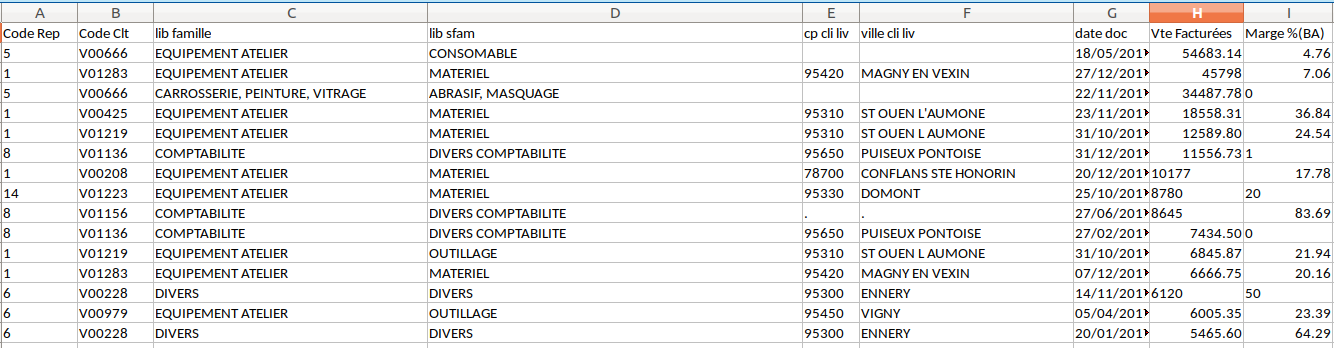
\includegraphics[scale=0.35]{img/data.png}
		\caption{Exemple de données fournies par VDSA}
	\end{center}
\end{figure}

De celles-ci nous en avons déduis les entités : Client, Commande, Article, Famille, Sous-Famille.
Un client possède un code (Code Clt), une adresse, un code postal (cp cli liv) et une ville (ville cli liv). Une commande est composée d'un identifiant, d'une date (date doc), d'un lieu, d'une marge (Marge\%(BA)) et d'un chiffre d'affaire. Un article a un identifiant et une date d'achat. Une famille possède une code pour l'identifer et d'un libellé (lib famille). Une sous-famille comprend un code pour l'identifier et d'un libellé (lib sfam).\\
De plus, notre site devra gérer des comptes utilisateur. Ainsi nous avons en plus créé l'entité Utilisateur. Celle-ci est constituée d'un identifiant, d'un nom, d'un prénom, d'un mail et d'un mot de passe. L'utilisateur aura également un rôle (exemple : administrateur). \\ \\
\noindent
Vous trouverez sur la page suivante le modèle conceptuel de nos données.

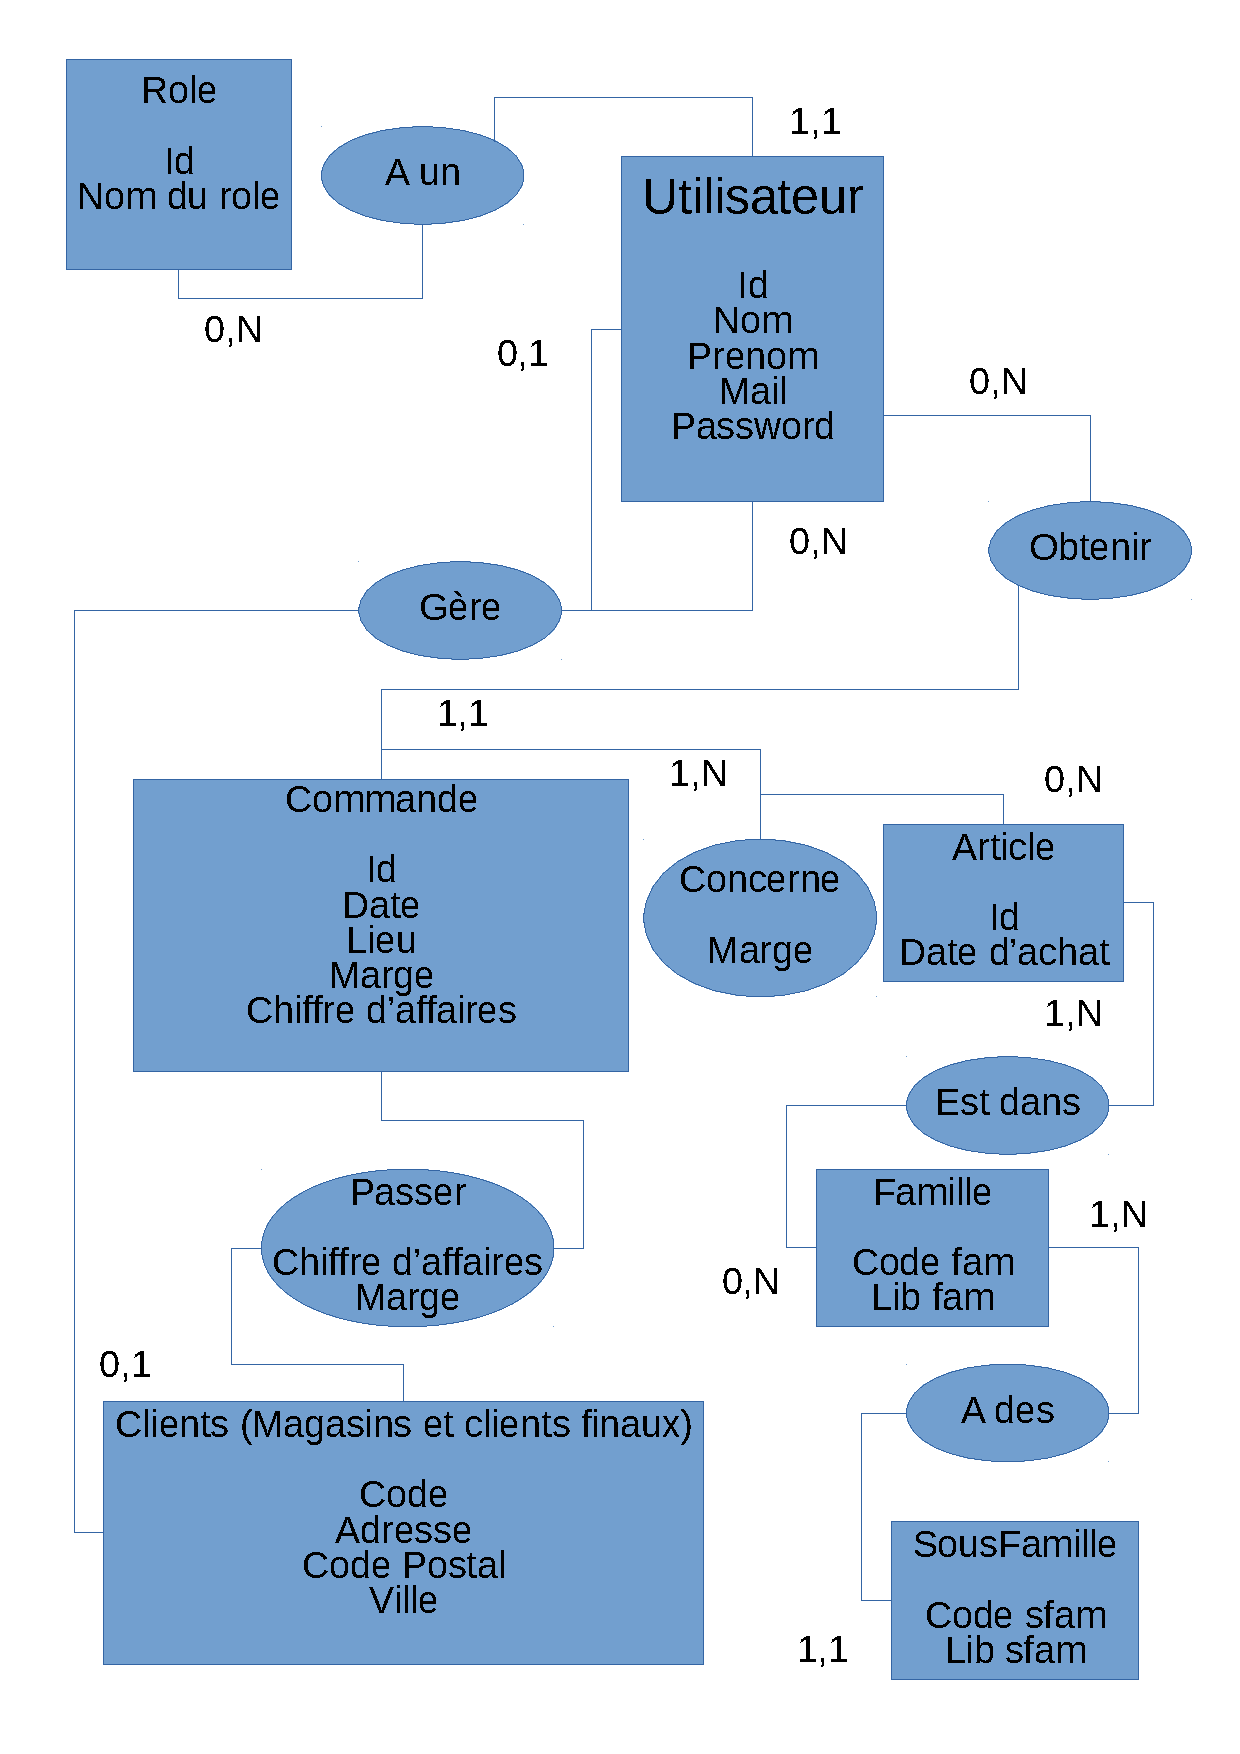
\includepdf{mcd.pdf}